\documentclass{article}
\usepackage{titlesec}
\usepackage[a4paper,margin=2.5cm]{geometry}
\usepackage{lmodern}
\usepackage{amsmath}
\usepackage{float}
\usepackage[dvipdfmx]{graphicx}
\usepackage{caption}

\begin{document}

\title{第2回輪講資料 『パワーエレクトロニクス入門』 pp.13-24, 94-124, 129-130}
\author{著者: 河村篤男 \\ 担当: 脇本 怜奈}
\date{\today}
\maketitle

\section*{概要}

\setcounter{section}{0}
\renewcommand{\thesection}{2.\arabic{section}}

\section{電力増幅と電力変換の相違点と共通点}

\section{可変抵抗を用いた電力変換の原理とその効率}
 電力変換器の入出力電力が図2.2のように考えられる場合、変換器の効率\(\eta\)は式(2.1)で表すことが可能である。\\
 \begin{align}
    \eta &= \frac{P_{out}}{P_{in}} \\
      &= \frac{P_{in} - P_{loss}}{P_{in}} = \frac{P_{out}}{P_{out}+P_{loss}}
\end{align}
 電力変換について、直流\(a\)[V]を直流\(b\)[V] (a \(>\) b)に変換することを考える。もっとも単純な回路の形は図2.3のようなものであり、出力電圧を\(b\)[V]に下げるためには\(a-b\)[V]に可変抵抗の電圧降下を設定すれば良い。回路に流れる電流は同一であるので、この電流を\(I\)とすると効率\(\eta\)は
\begin{align}
    \eta &= \frac{P_{out}}{P_{in}} = \frac{b\times I }{a \times I} = \frac{b}{a}
\end{align}
 電力変換の立場では効率100\(\%\)が理想とされることを考えると、この方法で電力変換を行うことは低効率である。

\section{スイッチを用いた電力変換の原理とその効率}
 続いて、理想スイッチ(オフ時は完全に電流を遮断し、オン時は短絡するようなスイッチ)を用いると、図2.3は図2.5(a)のようになる。図2.5(b)のように一定の周期でオンオフを切り替えると、
\begin{align}
    V_{av} &= \frac{T_{on}}{T_{SW}}E
\end{align}
ここで、オンオフの周期であるスイッチング周期は\(T_{sw}\)、スイッチがオンの期間は\(T_{on}\)、スイッチがオフの期間は\(T_{off}\)である。また、スイッチング周期に対するオン期間はデューティー比と定義でき、
\begin{align}
    d &= \frac{T_{on}}{T_{SW}}
\end{align}
となることから、この値を変化させることで平均電圧を調整できる。これをデューティー比制御、またはパルス幅制御(PWM)と呼ぶ。しかし、実際のスイッチにおける状況を考えてみると、図2.6に示すように電気的特性が異なる。\\
\\
\begin{tabular}{lrr} \hline
    & 理想のスイッチ & 実際のスイッチ \\ \hline
   オンオフ信号への応答 & 信号と同時に切り替わる & オンオフの切り替えに遅れが生じる\\
   オンオフ切り替え時の動作 & 瞬時に切り替わる & 切り替えに一定の時間がかかる\\
   オン時の電圧 & 抵抗0(完全に短絡) & 電圧降下が残る\\
   オフ時の電流 & 抵抗無限大(電流は0) & 小さな電流が流れる(ほとんどは無視できる)\\ \hline
\end{tabular}
\vspace{1em}
\\
 図2.6の上から4番目のグラフはスイッチにおける瞬時消費電力を示していて、切り替え時に大きな電力消費が発生する。オン時の電流を\(I_{SWon}\), 電圧を0, 切り替え時間を\(\delta T_{on}\), 電圧電流の変化を直線上であると近似して\\
\begin{align}
    i &= \frac{I_{SWon}}{\delta T_{on}}t \\
    v &= \frac{V_{SWoff}}{\delta T_{on}}(\delta T_{on} - t)
\end{align}

スイッチ状態の変化1回あたり発生する損失は、スイッチがオフからオンになるとき
\begin{align}
    W_{SW} = \int_{0}^{\delta T_{on}}vidt = \int_{0}^{\delta T_{on}}\frac{I_{SWon}V_{SWoff}}{\delta {T_{on}}^2}t(\delta T_{on} - t)dt = \frac{I_{SWon}V_{SWoff}}{6}\delta T_{on}
\end{align}
スイッチがオンからオフに切り替わる時は\(\delta T_{on}\)を\(\delta T_{off}\)とすれば良い。

1秒あたりのスイッチ回数、スイッチング周波数を\(f_{SW}\)と仮定する。スイッチ1回あたりの損失を\(W\)とすると、\(W\)は図2.6、図2.8に示す\textcircled{\scriptsize 1}から\textcircled{\scriptsize 4}の和であり、
\begin{align}
    W &= W_1 + W_2 + W_3 + W_4 \\
      &= \frac{I_{SWon}V_{SWoff}}{6}\delta T_{on} + I_{SWon}V_{SWon}T_{on} + \frac{I_{SWon}V_{SWoff}}{6}\delta T_{off} + I_{SWoff}V_{SWoff}T_{off}
\end{align}
1秒あたりに\(f_{SW}\)回オンオフが繰り返されるので、1秒あたりの損失である平均消費電力を\(P_{loss}\)とすると、
\begin{align}
    P_{loss} = Wf_{SW}=(W_1 + W_2 + W_3 + W_4)f_{SW}
\end{align}
先に定義したデューティー比を用いると、
\begin{align}
    P_{loss} = \frac{I_{SWon}V_{SWoff}}{6}(\delta T_{on} + \delta T_{off})f_{SW} + dI_{SWon}V_{SWon} + (1-d)I_{SWoff}V_{SWoff}
\end{align}
ここで、第一項はスイッチの切り替わり時に発生する損失で、1秒間にスイッチング周波数の回数発生する。この損失をスイッチング損失と呼ぶ。

\setcounter{section}{0}
\renewcommand{\thesection}{4.\arabic{section}}

\section{インバータの種類}
 インバータは、直流電圧源を入力側に持つ電圧形インバータと直流電流源を入力側に持つ電流形インバータに分類できる。

\section{電圧形インバータの基本回路と基本動作}

\section{単相電圧形インバータ}
 単相電圧形インバータは、整流したあとの直流電圧から単相商用交流電圧を生成する用途に主に用いられる。
\subsection{ハーフブリッジインバータ}

\subsection{フルブリッジインバータ}
 フルブリッジインバータは、基本回路のレグを二つ並列に接続し、その出力端子間に負荷を接続したものである。図4.12に動作モードを示す。
\begin{figure}[H]
    \centering
    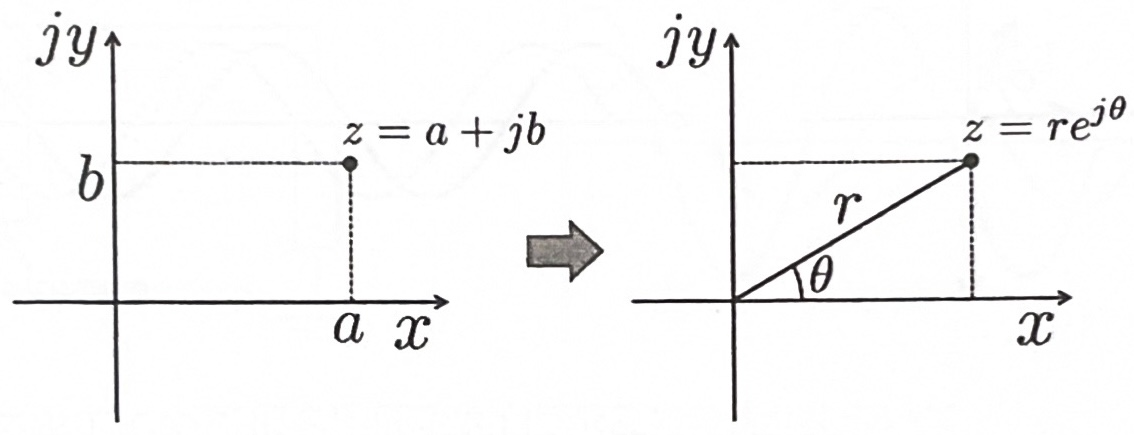
\includegraphics[width=0.5\textwidth]{images/2_26.jpg}
    \caption{図 2.34: 時間軸方向に平行移動した図2.33の系}
    \label{fig:2.34}
\end{figure}
スイッチ\(S_1\), \(S_2\)のオンオフ信号に対してスイッチ\(S_3\), \(S_4\)のオンオフ信号を\(\pi - \alpha \)遅らせた場合の\(\alpha \)を位相シフト量という。位相シフト量\(\alpha \)を変化させる制御法をパルス幅制御と呼ぶ。

\section{三相電圧形インバータ}
 三相電圧形インバータの回路図を図4.16に示す。
\begin{figure}[H]
    \centering
    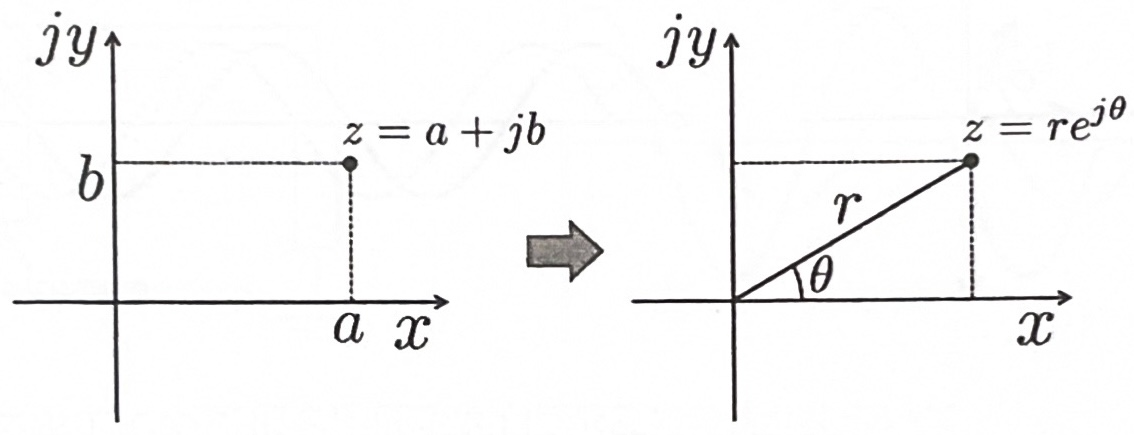
\includegraphics[width=0.5\textwidth]{images/2_26.jpg}
    \caption{図 2.34: 時間軸方向に平行移動した図2.33の系}
    \label{fig:2.34}
\end{figure}


\section{その他のインバータ回路}

\section{出力電圧の振幅制御方法}


\setcounter{section}{7}
\renewcommand{\thesection}{4.\arabic{section}}

\section{モータドライブ}

\setcounter{subsection}{1}
\renewcommand{\thesubsection}{\thesection.\arabic{subsection}}

\subsection{永久磁石同期電動機の制御}
 永久磁石同期電動機には、回転し構造により、図4.39(a)に示す表面磁石同期電動機と図4.39(b)に示す埋込磁石同期電動機に分類される。

\begin{figure}[H]
    \centering
    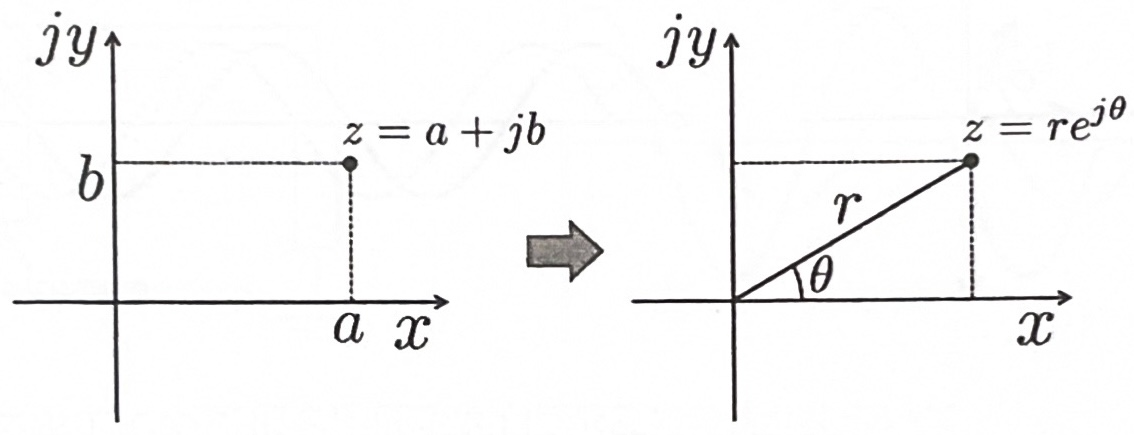
\includegraphics[width=0.5\textwidth]{images/2_26.jpg}
    \caption{図 2.34: 時間軸方向に平行移動した図2.33の系}
    \label{fig:2.34}
\end{figure}

いずれも回転子の磁極位置を検出または推定したうえで磁極位置に同期した座標系上に回転座標変換を行うと、基本波成分を直流で扱うことができるので制御が容易になる。
 



















\end{document}